\documentclass[10pt]{article}
\usepackage[margin=18mm]{geometry}
\usepackage[T1]{fontenc}
\usepackage{lmodern,graphicx,amsmath,amssymb,booktabs,longtable}
\usepackage[hidelinks]{hyperref}
\usepackage{microtype}
\emergencystretch=3em
\setlength{\parindent}{0pt}
\setlength{\parskip}{5pt}
\title{APS single-relation baseline and extensions}
\author{Crypto research implementation and correctness review}
\date{26 October 2026}
\begin{document}
\begin{center}
{\Large\bfseries APS single-relation baseline and extensions}\\[5pt]
Crypto research implementation and correctness review\\
26 October 2026
\end{center}
\textbf{Status: bounded native correctness; performance validation remains open.}
This report accompanies \texttt{research/aps\_extensions\_20261026/README.md},
\texttt{TRACKER.md}, \texttt{SOURCES.md} and the validation receipts.
It does not reproduce the paper's 11--22-bit parameter ladder or make a
performance, asymptotic, or deployed-curve-security claim.

\section*{Implemented path}
APS constructs known combinations $R_i=u_iG+v_iQ$ and solves a signed zero
sum using $S_m=0$. This differs from the conventional many-relation
$S_{m+1}(\ldots,x(R))=0$ route. Native F4 and curve arithmetic are reused.
After decoding, the code checks the point sum, rejects $B=0$ in
$AG+BQ=O$, and verifies $(-A/B)G=Q$. No target scalar, log table,
decomposition oracle or generic fallback is passed into relation solving.

\begin{center}
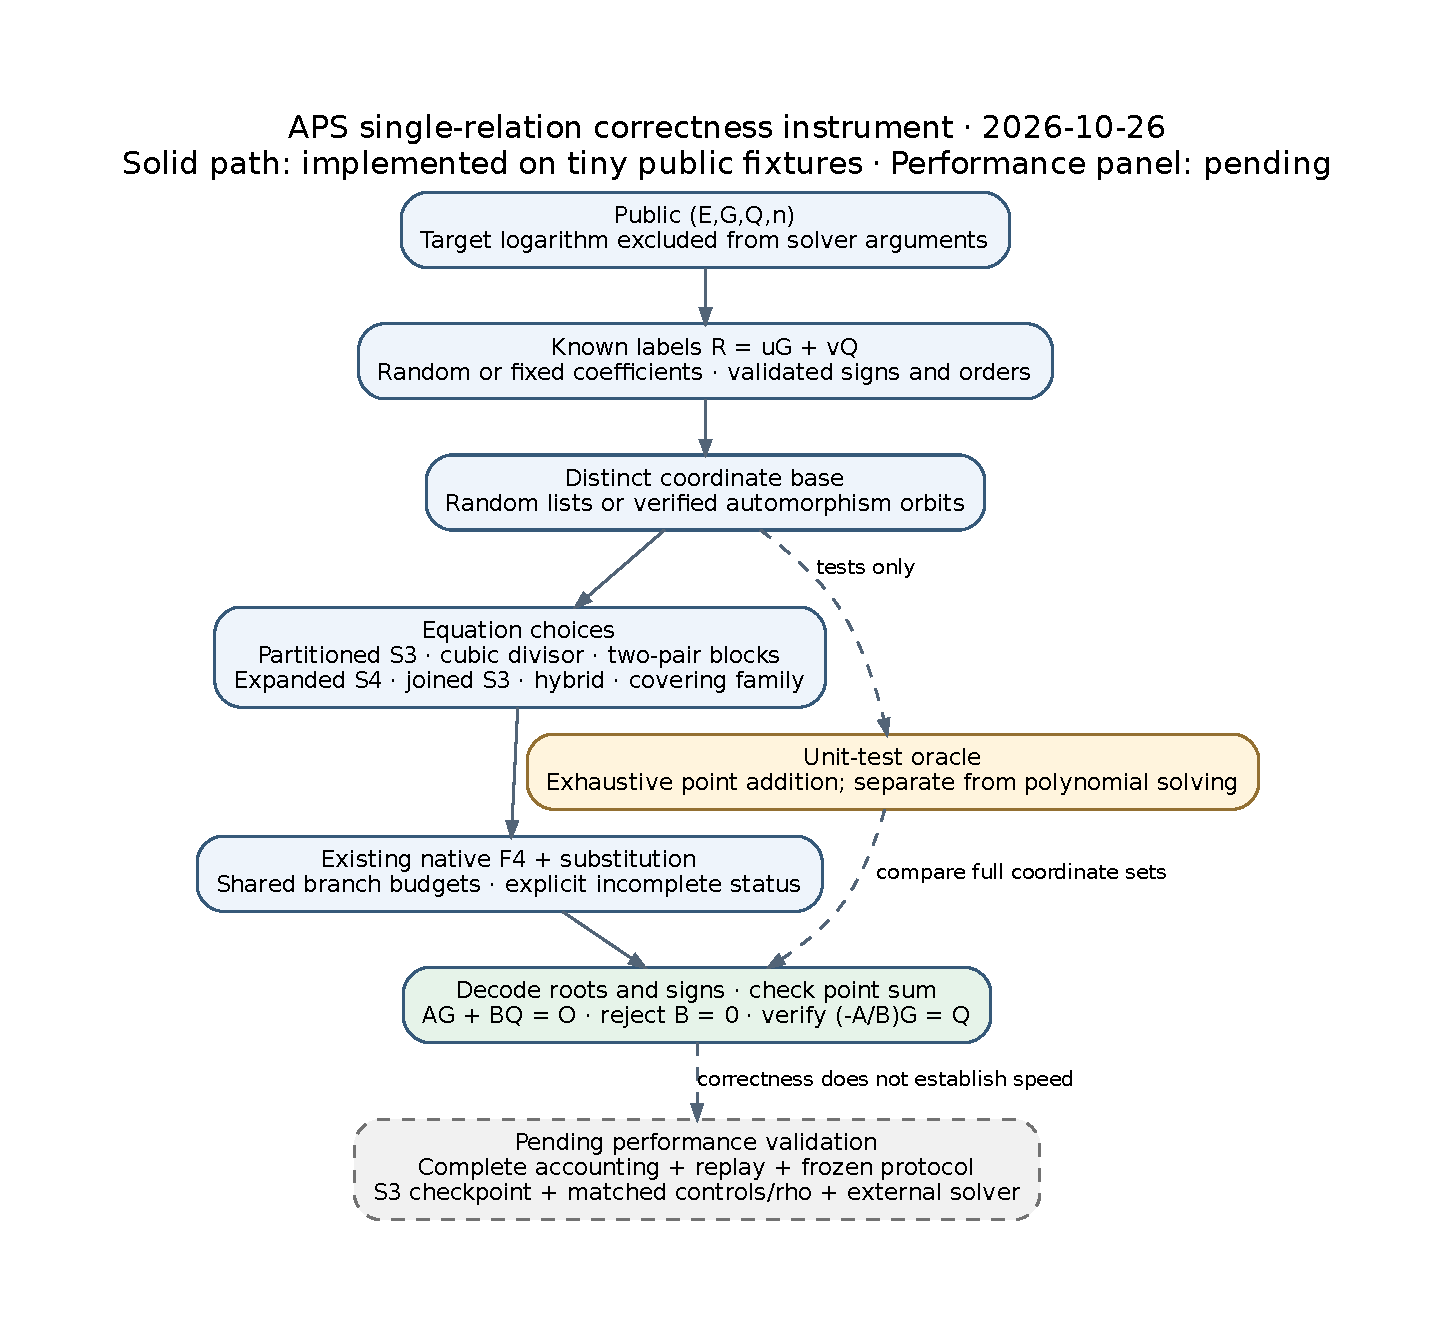
\includegraphics[width=0.96\linewidth,height=0.44\textheight,keepaspectratio]{pipeline.pdf}
\end{center}
\textbf{Figure 1.} Implemented correctness path and the separate test oracle.
No comparable controlled performance measurements exist for this study, so
the figure is a process diagram rather than a quantitative performance graph.

\newpage
\section*{Five tracked mechanisms}
\begin{description}
\item[APS-E1: coefficient labels.] Odd arity uses $v_i=1$ with $n>m$.
Even arity uses $1,2,4,\ldots$ with $n>\sum_i v_i$, one point per original
partition. Canonical sign changes propagate to labels. Orbit expansion and
even-arity block regrouping do not inherit the guarantee; $B\ne0$ is checked.
\item[APS-E2: unordered divisors.] A squarefree base polynomial is divisible
by $H(T)=T^3-e_1T^2+e_2T-e_3$ exactly when $H$ selects distinct base
coordinates. The established symmetric S3 rewrite is
$(e_2-a)^2-4e_1(e_3+b)=0$. A two-pair block variant is also implemented.
Remainder construction and equation degrees can cost more; no advantage is inferred.
\item[APS-E3: automorphism orbits.] The $j=0$ fixture verifies
$\phi(x,y)=(\beta x,y)$ and the subgroup eigenvalue before propagating labels.
Sparse constraints are retained. The intrinsic orbit relation has $A=B=0$
and is rejected. Related GLV folding is existing work in this repository.
\item[APS-E4: covering partitions.] A deterministic bit-based family separates
every distinct triple without inspecting relations. Its pre-deduplication
bound is $2\lceil\log_2 s\rceil(\lceil\log_2 s\rceil-1)$ colorings.
The family is not claimed balanced or optimal. Every solve shares one
deadline and duplicate coordinate sets count once.
\item[APS-E5: solver presentation.] Expanded S4, joined S3 and first-coordinate
hybrid guessing share a checked relation path. Joined S3 is already APS's
four-point baseline; hybrid and symmetry improvements have prior literature.
\end{description}

\section*{Correctness evidence and formal scope}
The 15 module tests pass in the isolated native review build; final integrated
checks are recorded in \texttt{validation/README.md}. Tests compare complete
coordinate sets with direct point addition and cover all encodings' public
DLP routes, labels, automorphism tautologies, coverage, invalid inputs and
timeouts. The point oracle is independent of polynomial construction but
shares the native curve arithmetic.

Public fixtures are:
\begin{center}
\begin{tabular}{rrrrrr}
\toprule
$p$ & $a$ & $b$ & $n$ & $G$ & public $d$\\
\midrule
101 & 59 & 6 & 107 & $(78,4)$ & 37\\
211 & 166 & 158 & 227 & $(155,121)$ & 73\\
103 & 0 & 5 & 97 & $(2,42)$ & 17\\
\bottomrule
\end{tabular}
\end{center}
The runner records full ICV1 identities. The field cap is 65521; the actual
tests are tiny. Native substitution may enumerate field values.

The pinned Lean proof gate audits 16 theorems, including generated equations,
with zero failing and zero trusted declarations. Eight named lemmas establish
integer parity, signed-one bounds and modular nonvanishing under stated
bounds. The power-sum magnitude bound remains a hypothesis. The elliptic-curve
bridge and Rust correspondence are tested, not formalized. The native
identity certificate checks S3 over its specified field and with an extra seed;
it is not a universal formal proof over all characteristics.

\section*{What remains open}
The F4 multiplication counter excludes complete setup, expression construction,
point arithmetic, decoding, duplicate handling and verification. Its degree
is top-level productive degree, not a substitution-tree maximum. Complete
accounting, independent transcript replay, ecbench/export integration,
preregistered held-out panels, matched strongest rho and an external polynomial
solver comparison remain open. Arbitrary composed-map bases and $m=5$ are
not implemented. No leaderboard row is promoted.

The documented container-local Conductor setup supplies the scoped reservation.
No S3 upload credential is available; no benchmark panel was launched.
Builds, unit tests and proof checking are ordinary validation. The tracker
preserves the larger request and acceptance criteria.

\section*{Sources and reproducibility}
APS, \emph{On the discrete logarithm problem for prime-field elliptic curves},
2018, \href{https://eprint.iacr.org/2017/609}{ePrint 2017/609}, revised author
manuscript, \S\S3.1--3.4. Full body read; solver complexity is explicitly unresolved.
Petit--Kosters--Messeng, PKC 2016, full author manuscript: composed-map prior work.
Galbraith--Gebregiyorgis, INDOCRYPT 2014, characteristic-two disjoint-base and
invariant-variable prior work.
Kudo--Yokota--Takahashi--Yasuda, CANS 2018,
\href{https://doi.org/10.1007/978-3-030-00434-7_19}{DOI 10.1007/978-3-030-00434-7\_19}:
official metadata/abstract checked; full-text gap, so no exact reproduction or
novelty claim. Exact links, hash and repository source map are in \texttt{SOURCES.md}.

\begin{verbatim}
cargo test --release --locked --lib aps_single_relation
cargo test --release --locked --example aps_single_relation_check
tools/lean/proof-gate.sh \
 research/aps_extensions_20261026/lean/Coefficients.lean
\end{verbatim}
The panel design is \texttt{PROTOCOL\_PLAN.md}; it is not a frozen protocol.
Detailed command outcomes, known integration blockers and receipts live in
\texttt{validation/README.md}. The Markdown record remains authoritative
for final validation status.
\end{document}
